
\section{The Physical System and Modeling}
\begin{frame}
  \begin{itemize}
	\item Mathematical models are an abstraction of reality.
	\item There are three types of responses. 
	\begin{enumerate}
		\item Linear\\
		$\ y'=\alpha y$
		\item Exponential\\
		$\ y' = \frac{\alpha y}{y+ L}$ 
		\item Logistic\\
		$\ y'= \frac {\alpha y^2}{\beta + y^2}$
	\end{enumerate}
  \end{itemize}
\end{frame}

\begin{frame}
  \frametitle{Type I Response}
   Linear: $y'=\alpha y$\\ Applied to phenomena including chemical reaction kinetics.
   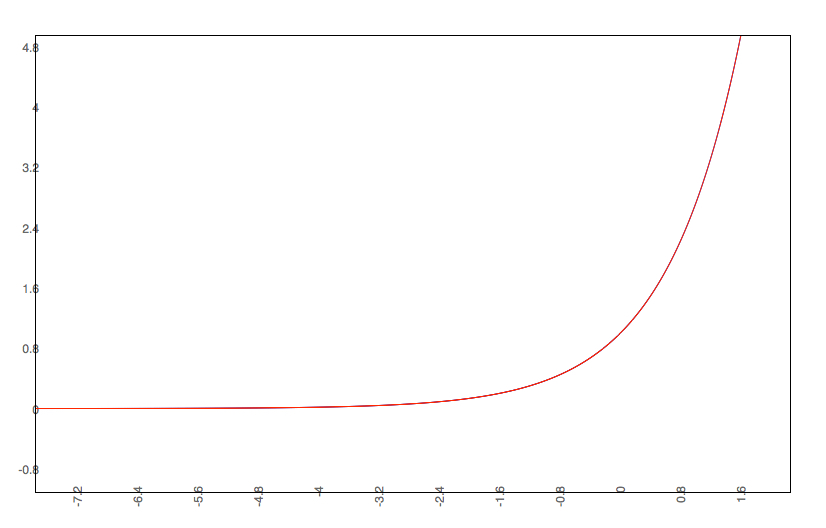
\includegraphics[scale=.4]{typeI}
\end{frame}

\begin{frame}
  \frametitle{Type II Response} Models population growth until carrying capacity is reached.
    Type II: $y'=\frac{\alpha y}{y+L}$
   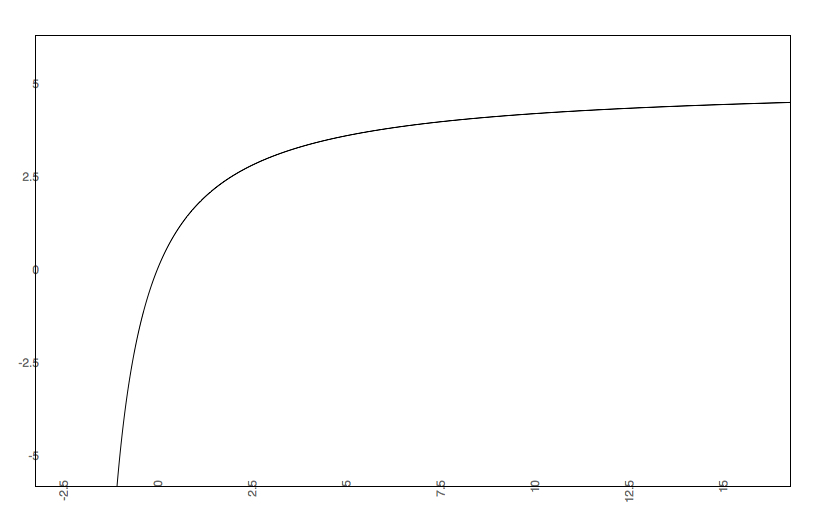
\includegraphics[natwidth=162bp, natheight=227bp,width=280bp]{typeII.jpg}
\end{frame}

\begin{frame}
  \frametitle{Type III Response}
    Logistic Curve: $y=\frac{15}{1+e^{-x}}$. Used to model neuronal action potentials.
    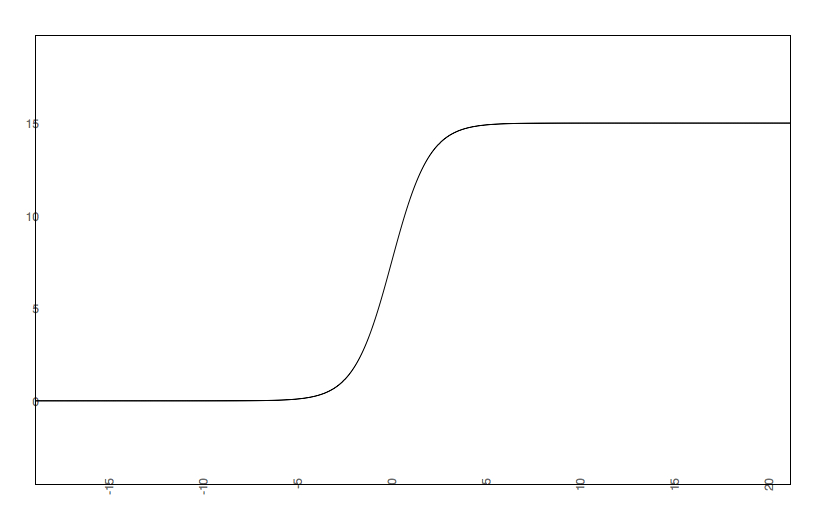
\includegraphics[scale=.4]{typeIII.jpg}
\end{frame}

\begin{frame}
\frametitle{Coral Reef Dynamics}
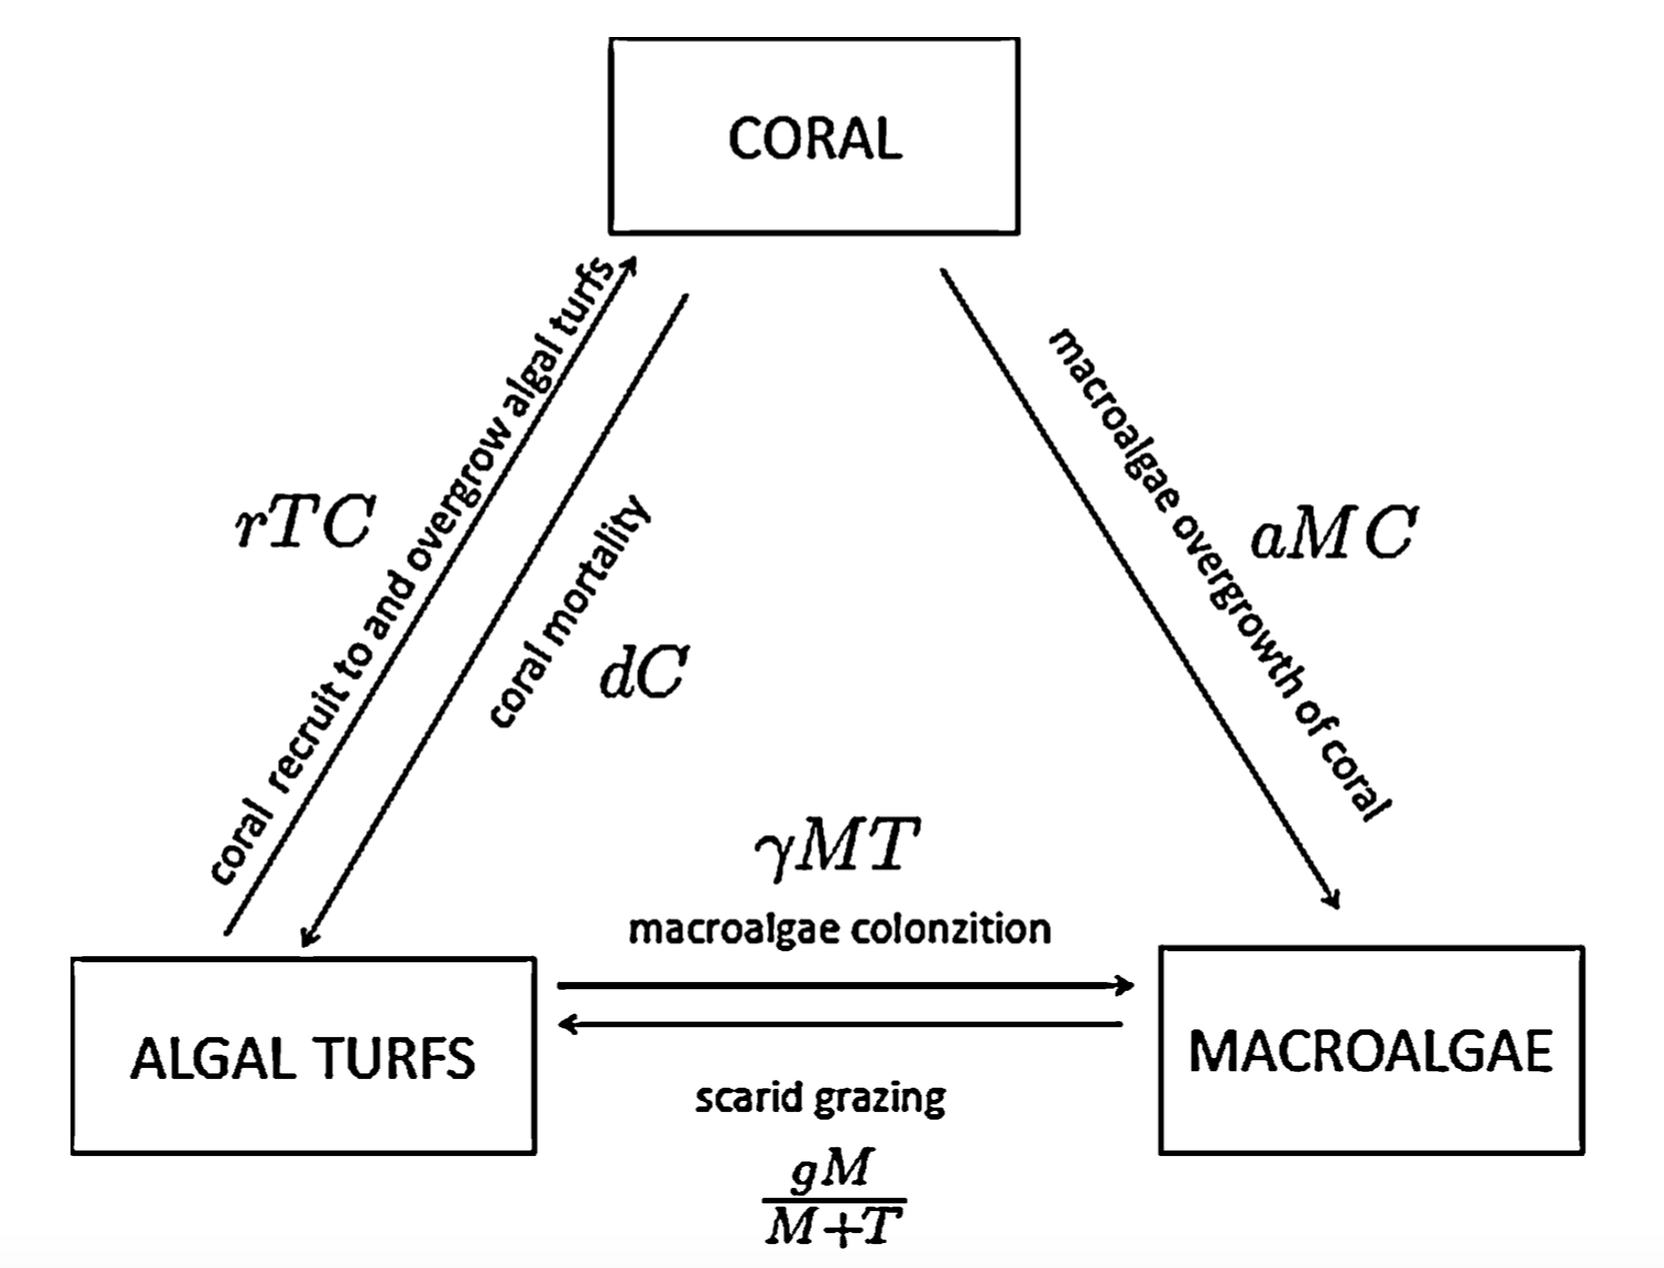
\includegraphics[natwidth=162bp,natheight=227bp,width=280bp]{./coral-reef-triangle.png}
\end{frame}
\begin{frame}
$$\begin{cases}\begin{array}{rl}
\frac{dM}{dt}\hspace{-.8em}&=aMC - \frac{gM}{M+T}+\gamma M T\\
\frac{dC}{dt}\hspace{-.8em}&=rTC - dC - aMC\\
\frac{dT}{dt}\hspace{-.8em}&=\frac{gM}{M + T} - \gamma MT - rTC + dC
\end{array}\end{cases},$$ where \begin{itemize}\itemsep0pt
\item $r$ is the rate corals overgrow upon algal turfs\\
\item $d$ is the mortality rate of corals\\
\item $a$ is the rate that macroalgae overgrow upon corals\\
\item $\gamma$ is the rate that macroalgae spread over algal turfs\\
\item $g$ is the indiscriminate grazing rate of parrotfish.
\end{itemize}
\end{frame}

\begin{frame}
If we restrict our scope to regions entirely covered by coral, macroalgae, and algalturf, we may suppose that $M+C+T=1$ implying that  $\frac{dT}{dt}=-\frac{dM}{dt}-\frac{dC}{dt}$. This substitution allows us to  reduce our system to, $$\begin{cases} 
\begin{array}{rl}
\frac{dM}{dt}&= aMC-\frac{gM}{M+T} + \gamma MT\\ 
\frac{dC}{dt}&=rTC-dC-aMC
\end{array} \end{cases}.$$ 
\end{frame}

\begin{frame}
  \frametitle{Nondimensionalization}
  To simplify systems of equations we scale problems using the technique of nondimensionalization: set {\begin{itemize}\itemsep0pt\item $M(t)=\overline{M}\HAT{M}(s)$;\\\item $C(t)=\overline{C}\HAT{C}(s)$;\\\item $T(t)=\overline{T}\HAT{T}(s)$, and;\\\item $t=\tau s$. \end{itemize} From this we get: \begin{itemize}\itemsep0pt \item$\frac{dM}{dt}=\overline{M}\HAT{M}'\frac{ds}{dt}$;\\\item $\frac{dC}{dt}=\overline{C}\HAT{C}'\frac{ds}{dt}$;\\\item $\frac{dT}{dt}=\overline{T}\HAT{T}'\frac{ds}{dt}$, and;\\ $\frac{ds}{dt}=\frac{1}{\tau}.$\end{itemize} }Our system then becomes: $$\begin{cases} 
\begin{array}{rl}
\frac{\overline{M}}{\tau}\frac{d\HAT{M}}{dt}&= a\overline{M}\overline{C}\HAT{M}\HAT{C}-\frac{g\overline{M}\HAT{M}}{\overline{M}\HAT{M}+\overline{T}\HAT{T}} + \gamma \overline{M}\HAT{M}\overline{T}\HAT{T}\\ 
\frac{\overline{C}}{\tau}\frac{d\HAT{C}}{dt}&=r\overline{T}\overline{C}\HAT{T}\HAT{C}-d\overline{C}\HAT{C}-a\overline{M}\overline{C}\HAT{M}\HAT{C}
\end{array} \end{cases}$$
\end{frame}
{\center
\begin{frame}$$\begin{cases}
\begin{array}{rl}
\frac{\overline{M}}{\tau}\frac{d\HAT{M}}{dt}&= a\overline{M}\overline{C}\HAT{M}\HAT{C}-\frac{g\overline{M}\HAT{M}}{\overline{M}\HAT{M}+\overline{T}\HAT{T}} + \gamma \overline{M}\HAT{M}\overline{T}\HAT{T}\\ 
\frac{\overline{C}}{\tau}\frac{d\HAT{C}}{dt}&=r\overline{T}\overline{C}\HAT{T}\HAT{C}-d\overline{C}\HAT{C}-a\overline{M}\overline{M}\HAT{C}\HAT{C}
\end{array} \end{cases}$$$$\begin{cases}
\begin{array}{rl}
\frac{d\HAT{M}}{dt}&= a\tau\overline{C}\HAT{M}\HAT{C}-\frac{g\tau\HAT{M}}{\overline{M}\HAT{M}+\overline{T}\HAT{T}} + \gamma \tau\HAT{M}\overline{T}\HAT{T}\\ 
\frac{d\HAT{C}}{dt}&=r\tau\overline{T}\HAT{T}\HAT{C}-d\tau\HAT{C}-a\tau\overline{M}\overline{C}\HAT{M}\HAT{C}
\end{array} \end{cases}$$$$\begin{cases}
\begin{array}{rl}
\frac{d\HAT{M}}{dt}&= \HAT{M}(a\tau\overline{C}\HAT{C}-\frac{g\tau}{\overline{M}\HAT{M}+\overline{T}\HAT{T}} + \gamma \tau\overline{T}\HAT{T})\\ 
\frac{d\HAT{C}}{dt}&=\HAT{C}(r\tau\overline{T}\HAT{T}-d\tau-a\tau\overline{M}\overline{C}\HAT{M}
\end{array} \end{cases}$$ Set $\overline{T}=\frac{r}{\gamma}$, $\overline{C}=\frac{r^2}{a\gamma}$, $\overline{M}={r^2}{a\gamma}$, $\tau=\frac{\gamma}{r^2}$.
\end{frame}
}
\begin{frame}$$\begin{cases}
\begin{array}{rl}
\frac{d\HAT{M}}{dt}&= \HAT{M}(\frac{a\gamma r^2}{r^2\gamma a}\HAT{C}+\frac{\gamma}{r}\HAT{T}+\frac{g\gamma}{r^2\HAT{M}+ \frac{r^3}{\gamma}\HAT{T}}) \\ 
\frac{d\HAT{C}}{dt}&=\HAT{C}(\frac{r^2\gamma}{r^2\gamma}\HAT{T}-\frac{a\gamma r^2}{r^2\gamma a}\HAT{M}-\frac{d\gamma}{r^2})
\end{array} \end{cases}$$$$\begin{cases}
\begin{array}{rl}
\frac{d\HAT{M}}{dt}&= \HAT{M}(\HAT{C}+\frac{\gamma}{r}\HAT{T}+\frac{g\gamma}{r^2\HAT{M}+ \frac{r^3}{\gamma}\HAT{T}}) \\ 
\frac{d\HAT{C}}{dt}&=\HAT{C}(\HAT{T}-\HAT{M}-\frac{d\gamma}{r^2})
\end{array} \end{cases}$$ Recall, \begin{itemize}\itemsep0pt
\item $r$ is the rate corals overgrow upon algal turfs\\
\item $d$ is the mortality rate of corals\\
\item $a$ is the rate that macroalgae overgrow upon corals\\
\item $\gamma$ is the rate that macroalgae spread over algal turfs\\
\item $g$ is the indiscriminate grazing rate of parrotfish.
\end{itemize}
\end{frame}

\begin{frame}
  \frametitle{Blood Coagulation}
  Blood coagulation in response to an injury occurs in three stages: \begin{itemize}
  \item Initiation stage: injury exposes tissue factor to the site of injury thereby initiating the coagulation process. TF + factor VII = TF-VIIa complex activates factors IX and X. X activates thrombin before plasma protease inhibitor (TFPI) binds to and inactivates TF, Xa, and finally TF-VIIa which terminates this stage.\\
  \item Amplification stage: thrombin activates platelets and factor V and VIII which drives the formation of a coagulation complex (IXa-VIIIa-Ca-PL, Xa-Va-Ca-PL) serving as an initial plug of the injury. TFPI inactivates thrombin terminating this stage.\\
  \item Propagation stage: increasing platelet production of thrombin leading to thrombin's cleavage of the initial plug's fibrinogen into fibrin to which the final plug owes its strength.
  \end{itemize}
\end{frame}

\begin{comment}

\begin{frame}\frametitle{Coagulation Cascade}
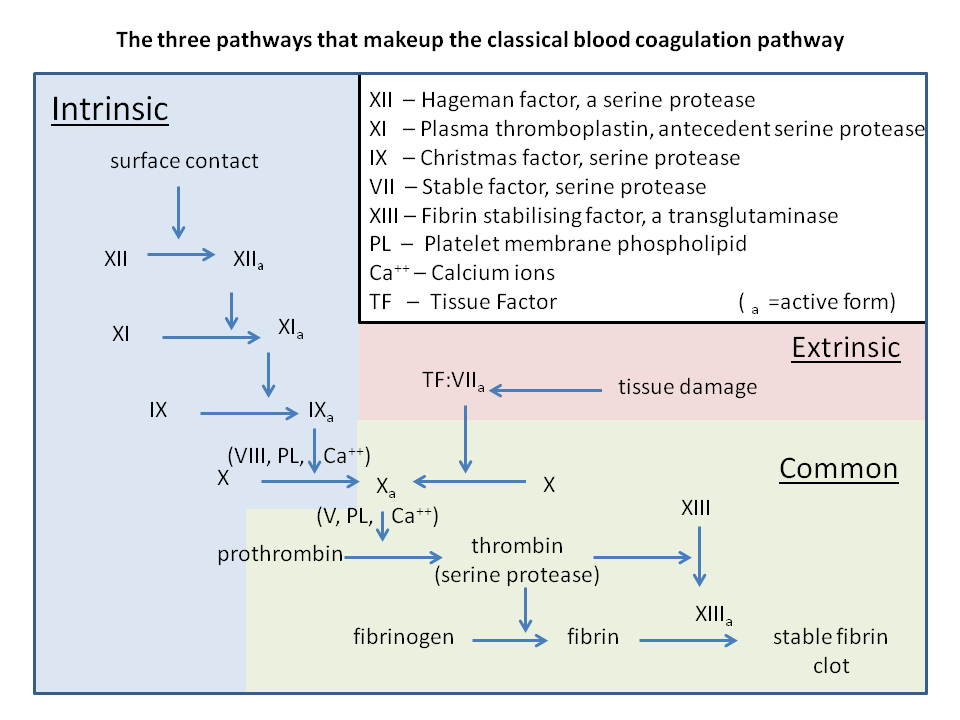
\includegraphics[natwidth=162bp,natheight=227bp,width=280bp]{./coag-cascade.png}
\end{frame}

\begin{frame}\frametitle{Clotting Factor Models}
\begin{itemize}
\item 1989 Khamin-Semenov Model - Treated Coagulation as a three stage process as previously described.\\
\item 2002 Xu Model extends the K-S Model to be more applicable to bleeding pathologies.\\
\item 2004 Qiao et. al. Model focuses on the role of activated protein C (factor XIV)
\end{itemize}
\end{frame}

\begin{frame}
\frametitle{1989 Khamin-Semenov Model}
$$\begin{cases}\begin{array}{rl}
\frac{dVIIa}{dt}\hspace{-.8em}&=\alpha k_1- H_4[VIIa]\\
\frac{dXa}{dt}\hspace{-.8em}&=k_2[VIIa]-H_2[Xa]\\
\frac{dVa}{dt}\hspace{-.8em}&=k_3[IIa]-H_3[Va]\\
\frac{dIIa}{dt}\hspace{-.8em}&=k_4[Xa]\frac{[Va]}{k_a+[Va]}-H_4[IIa]
\end{array}\end{cases},$$ where $\{k_i\}$ are kinetic coefficients and $\{H_i\}$ are dissipation constants. Xu notes that this model lacks the role that platelets play in this model.
\end{frame}
\end{comment} 


\begin{frame}
\frametitle{2002 Xu Model}\vspace{-1.5em}
$$\begin{cases}\begin{array}{rl}
\frac{d(TF-VIIa)}{dt}\hspace{-.8em}&=[TF-VIIa]_0-h'_1[TF-VIIa]([TFPI][Xa]k_{14})\\
\frac{dXa}{dt}\hspace{-.8em}&=k_2[TF-VIIa]+k_{21}[IXa]\left(\frac{VIIIa}{VIIIa+d_2}\right)\left(c_0+\frac{f(IIa)}{1+f(IIa)}\right)\\&\hspace{1em}-h'_{21}[TFPI][Xa]-h'_{22}[AT][Xa]\\
\frac{dIXa}{dt}\hspace{-.8em}&=k_3[TF-VIIa]-h'_3[AT][IXa]\\
\frac{dVa}{dt}\hspace{-.8em}&=k'_5[IIa][V]-h'_5[Va]\\
\frac{dVIIIa}{dt}\hspace{-.8em}&=k'_6[IIa][VIII]-h'_6[VIIIa]\\
\frac{dIIa}{dt}\hspace{-.8em}&=k_4[Xa]\frac{[Va]}{[Va]+d_1}\left(c_0+\frac{f(IIa)}{1+f(IIa)}\right)-h'_4[IIa]
\end{array}\end{cases},$$ where $\{k'_i\}$ are kinetic coefficients and $\{h'_i\}$ are dissipation constants.

\hspace{1.57em}The role that platelets have in this model is realized by the term $c=c_0+\frac{[IIa]}{1+[IIa]}$, the proportion of platelets that have be activated by thrombin.% (Xu asserts this is a strict, twice differentiable function of $[IIa]$ whose codomain is $[0,1]$).
\end{frame}
\begin{comment}
\begin{frame}
\frametitle{2004 Qiao et. al. Model}\vspace{-1.5em}
$$\begin{cases}\begin{array}{rl}
\frac{d[IXa]}{dt}\hspace{-.8em}&=k_1\beta-h_1[IX_a]\\
\frac{d[VIIIa]}{dt}\hspace{-.8em}&=k_2[IIa]+k_3[X_a]-k_4[APC]\frac{[VIIIa]}{b_1+[VIIIa]}-h_2[VIIIa]\\
\frac{d[Xa]}{dt}\hspace{-.8em}&=k_5[IXa]\frac{[VIIIa]}{b_2+[VIIIa]}-h_3[Xa]\\
\frac{d[Va]}{dt}\hspace{-.8em}&=k_6[IIa]-k_7[APC]\frac{Va}{b_3+Va}-h_4[V_a]\\
\frac{d[APC]}{dt}\hspace{-.8em}&=k_8[IIa]-h_5[APC]\\
\frac{d[IIa]}{dt}\hspace{-.8em}&=k_9[Xa]\frac{[Va]}{b_4+[Va]}-h_6[IIa]
\end{array}\end{cases},$$ where $\{k'_i\}$ are kinetic coefficients and $\{h'_i\}$ are dissipation constants.
\end{frame}

\begin{frame}\frametitle{Moiseyev and Friends' Random Fibrin Walk}
Basis for the model is the 1998 Keener-Snead model: $$\frac{\partial n}{\partial t}+V\frac{\partial n}{\partial x}=F(1-n)-Gn,$$ where \begin{itemize}\item$n(x,t)dx$ is the fraction of connected links in the interval $[x,x+dx]$ at time $t$;\item $F(x)$ is the rate of link formation; \item $G(x)$ rate of lin dissociation; \item $V$ is the velocity field representing a shear flow.\end{itemize}
\end{frame}
\end{comment}

%%% Local Variables:
%%% mode: latex
%%% TeX-master: "Presentation1"
%%% End:
